%----------------------------------------------------------------------------
\chapter{Előismeretek}
%----------------------------------------------------------------------------

%\section{Részleges modellek fajtái}
%\subsection{May}
%\subsection{Abs}
%\subsection{Var}
%\subsection{OW}
\section{Felvezetés}
%pl osztálydiagram

A részleges modellezést legegyszerűbben egy gyakorlati példán lehet bemutatni. Vegyük példának az UML \cite{UML} osztálydiagramját. Az UML (Unified Modeling Language) egy szabványos, objektumorientált modellezési nyelv, ami a tervezést, fejlesztést és egyéb folyamatokat segíti. Ezt a nyelvet informatikában és egyéb üzleti területeken egyaránt alkalmazzák. Magában foglal több diagram típust is.
\par
Az osztálydiagram egy strukturális diagram, segítségével egy rendszerben előforduló objektumokat, azok tulajdonságait és kapcsolatait lehet modellezni. Az objektumok téglalapokkal vannak jelezve, a hozzájuk tartozó attribútumok a téglalapon belül helyezkednek el és az elemek összekötésével a kapcsolatokat lehet jelezni. 
\par
Az alábbi példában (lásd \autoref{jarmu}) egy járműnek az osztálydiagramja látható. A járműnek vannak attribútumai és tartalmaz ajtót, kereket és üléseket, továbbá van neki egy meghajtása, ami egy absztrakt osztály. Ezek ugyan azon attribútumokkal van ellátva: id, típus, név. A meghajtásnak két leszármazottja van a benzinmotoros és a villanymotoros meghajtás. A benzinmotor tulajdonsága a hengerek száma a villanymotor tulajdonsága pedig az akkumulátor kapacitása.

\begin{figure}[!ht]
	\centering
	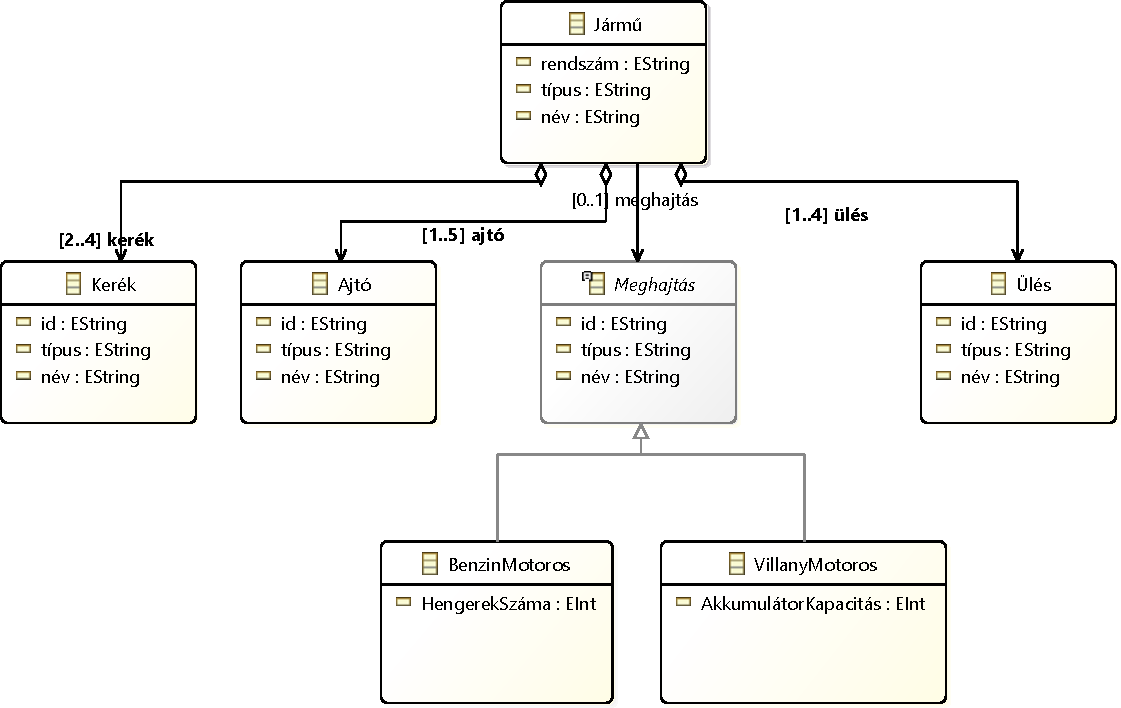
\includegraphics[width=130mm]{figures/vehicle.pdf}
	\caption{Jármű egyszerűsített osztálydiagramja} 
	\label{jarmu}
\end{figure}

\section{Részleges modell}
Részleges modell segítségével lehetőség van tervezői döntések dokumentálására. Általában a modellező eszközökkel csak érvényes modelleket lehet készíteni. Így a modell készítője belekényszerül olyan döntések meghozatalába, amiket csak később kéne meghozni, emiatt elveszhetnek tervezői döntések. Részleges modellben lehetőség van ezeket a kétséges helyzeteket már a modellezés szintjén kezelni. Így a modell nem csupán a struktúráról tartalmaz információt, hanem a részlegességről is, tehát hogy teljesen specifikált a modell vagy sem. 
\par
Az előbbi példát tekintve, lehetséges az hogy a járműnek egyáltalán nem szeretnénk ajtót, mert egy motort akarunk modellezni. Ekkor feleslegessé válik teljesen az ajtó jelenléte a modellben. Erről információt az UML szabályai szerint nem tudunk tárolni. Vagy feljegyezzük a lehetséges változtatást, vagy pedig létrehozunk egy másik diagramot, amibe van a járművön ajtó és egy olyat, amiben nincs. Ezek egyike sem tűnik jó megoldásnak. Egy ilyen picike diagram esetén még akár átlátható de egy nagyobb, akár több száz elemből álló modell esetén, ha máshol is van ilyen kétség a végleges modellel kapcsolatban, akkor már kezelhetetlenné válik. Például 5 ilyen döntés esetében 2\^5 darab diagramot kéne párhuzamosan fejleszteni.
\par
Lehetőség van a modell finomítására is (lásd \autoref{finomit}). Finomítás során a parciális modellből kikerülnek bizonytalan elemek. Ez azt jelenti, hogy a modellben jelzett részlegesség mértéke csökkenthető és ennek eredményeképpen véges számú finomítás után a modellből teljesen eltűnnek a részlegességek.

\begin{figure}[!ht]
	\centering
	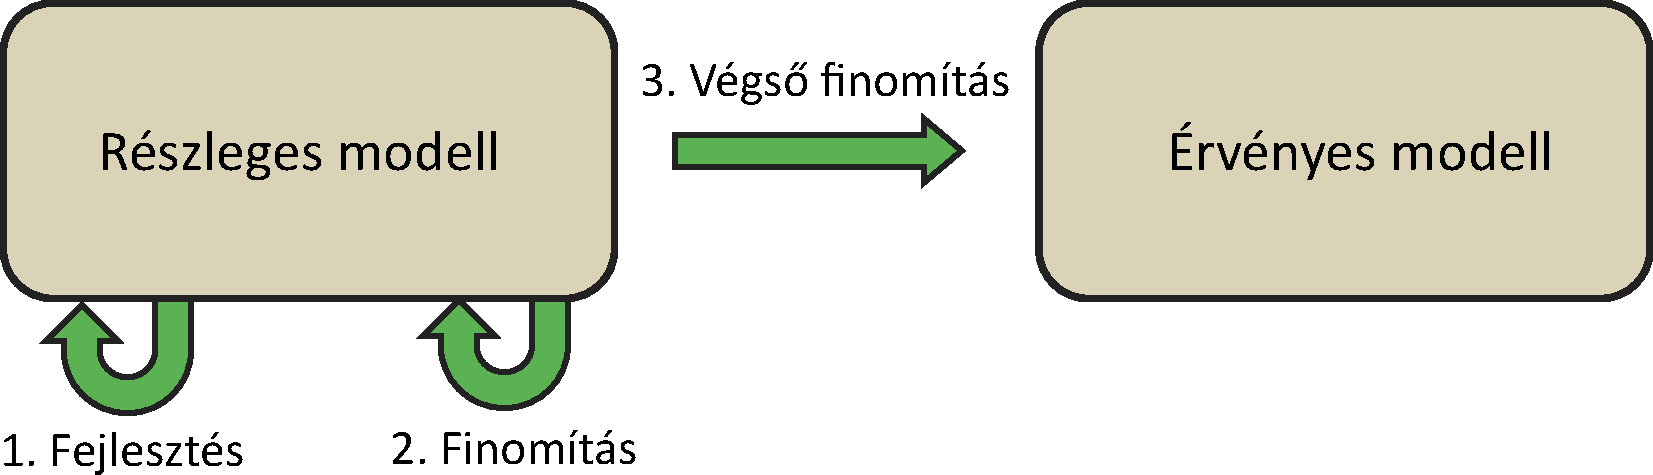
\includegraphics[width=130mm]{figures/finom.pdf}
	\caption{Finomítás menete} 
	\label{finomit}
\end{figure}

\subsection{Szintaktika}
Részleges modellek esetén annotációkkal lehet megjelölni a modellt, illetve annak elemeit. Modellezés során négy fajta részlegességet jelölhetünk meg \cite{Salay}. Annotációk a modell minden elemére kerülhetnek, lehet attribútumra, objektumokra, élekre vagy akár magára a modellre is.


\subsection{Szemantika}
\subsubsection{May}
Annotációkkal láthatjuk el a modellt az alapján, hogy egy modellelem biztosan benne lesz a végleges modellben, vagy pedig még bizonytalan a léte. \textsf{’M’} May exist (lehet, hogy benne lesz a végleges modellben, de lehet, hogy nem), \textsf{’E’} Must exist (biztosan benne lesz a végleges modellben). A modell finomításával lépésről lépésre egyre kevesebb ’M’ lesz.  \textsf{’M’} az vagy átvált \textsf{’E’}–re, vagy teljesen kikerül a modellből. Akkor tekinthető a modell véglegesnek, ha már nem szerepel benne \textsf{’M’}-el megjelölt elem. Továbbiakban az \textsf{’E’} jelöléssel nem foglalkozom, mert amelyik elemen nincs annotáció, az benne van a modellben.
\par
Tegyük fel, hogy nem tudjuk milyen járművet akarunk még modellezni a kezdeti fázisban. Ezért a kiindulási objektummodellben elláttuk May annotációkkal a járműnek az ajtó elemét. Így finomítás során ez az elem később eltűnhet de akár meg is maradhat. Az a jármű aminek nincs ajtaja lehet akár egy motor, a két ajtós változat pedig egy autó. Erre példa az alábbi diagramrészlet (lásd \autoref{may}).

\begin{figure}[htp]
	\centering
	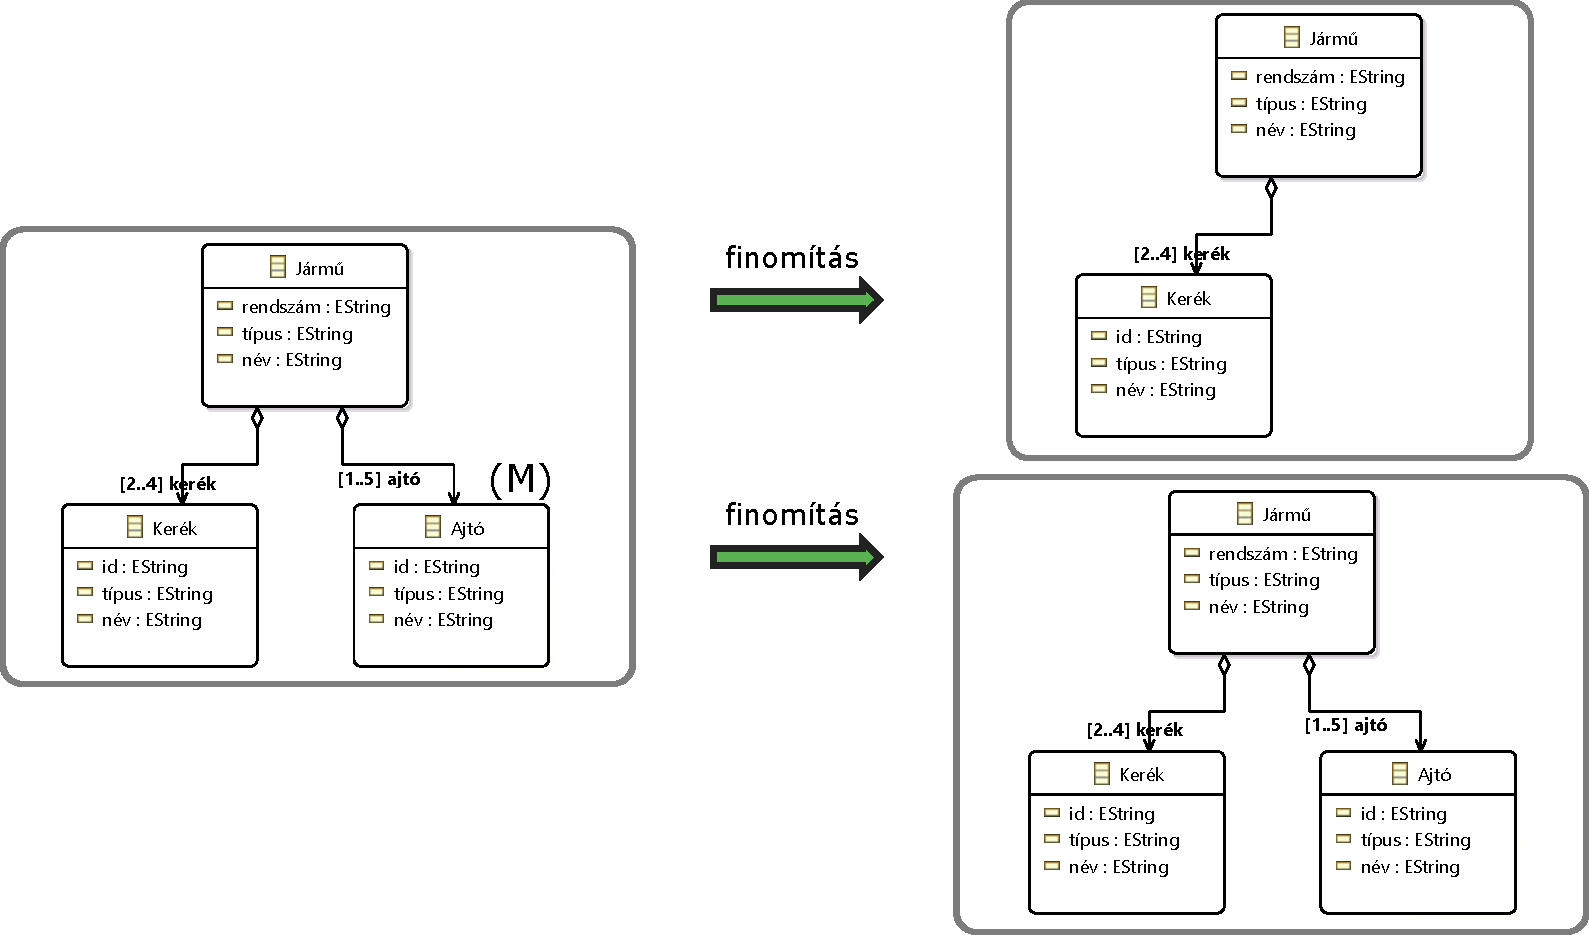
\includegraphics[width=130mm]{figures/may.pdf}
	\caption{May részlegesség feloldása} 
	\label{may}
\end{figure}

\subsubsection{Abs}
Ennek is két különböző annotálási módja lehet: \textsf{’P’}, Particular (egyedi elem) és \textsf{’S’}, azaz Set (egy vagy több elemet jelölhet). Particular az olyan elem, ami már biztosan benne lesz a végleges modellben, azonban a Set olyan elemet jelöl, ami legalább egyszer elő fog fordulni a végleges modellben, de lehetséges hogy többször is. Finomítások során az \textsf{’S’}-el megjelölt tagokat szétbontjuk több részre vagy meghagyhatjuk egyedi elemként, de a végleges modellben már csak egyedi elemek szerepelhetnek. Egyedi elem esetében az annotációt mellőzhetjük.
%Legyen 'e' a modellnek egy eleme S(e) egy Set annotációval megjelölt elem. Finomítás után ez az elem 'n' darab elemre válhat szét, ahol \in
\par
Diagram kezdeti fázisában még nincs eldöntve, hogy az ülés az egyedi elem vagy sem, ezért meg van jelölve egy \textsf{’S’} annotációval. Lehetséges, hogy egy együléses versenyautót szeretnénk építeni, de lehet, hogy egy családi autót, aminek van hátsó ülése is. Finomítás során az ülést megtartjuk eredeti formájában. A másik lehetőség viszont az, hogy szétbontjuk első illetve hátsó ülésre. Ebben az esetben ugyan azok a tulajdonságok lesznek meg mind a két ülésben (pl.: szín, anyaghasználat), de mégis modell szempontjából külön kezelendőek. Erre példa az alábbi diagramrészlet (lásd \autoref{abs}).

\begin{figure}[htp]
	\centering
	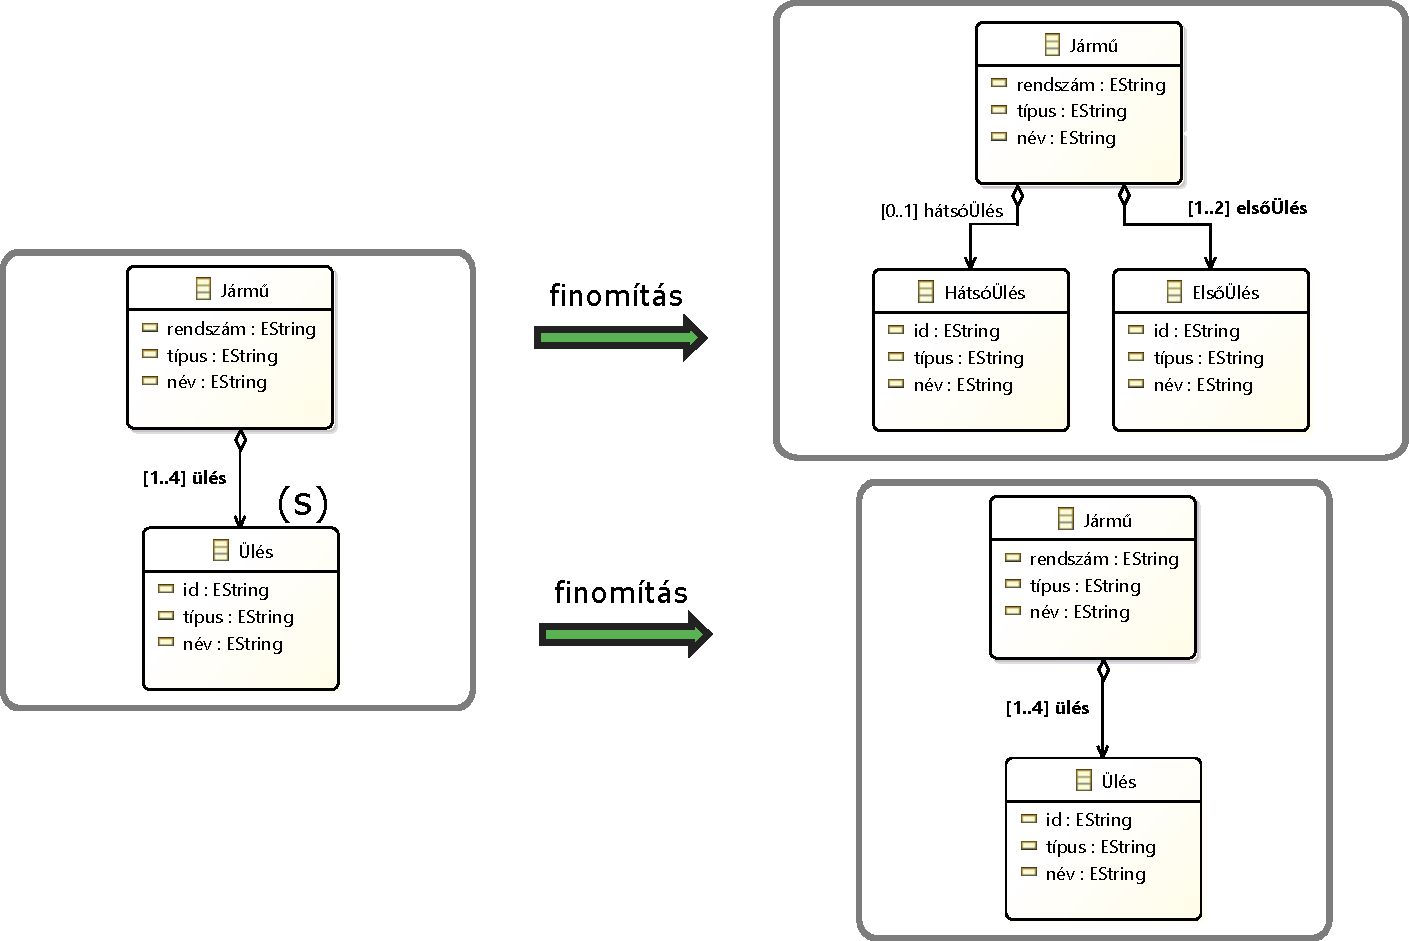
\includegraphics[width=130mm, keepaspectratio]{figures/abs.pdf}
	\caption{Abs részlegesség feloldása} 
	\label{abs}
\end{figure}

\subsubsection{Var}
Kétféleképpen lehet annotálni az elemeket: \textsf{’C’} Constant (konstans elem) és \textsf{’V’} Variable (változó elem). Bizonyos értelemben az Abs fordítottjának lehet tekinteni, mert nem elemeket többszöröz, hanem összeolvaszt. Felveszünk több elemet a modellbe, ami lehet, hogy későbbiekben összeolvasztunk egy elemmé, tehát fenn áll a lehetősége annak, hogy két elem megegyezik a modellezés első szakaszában. Amikor elkezdünk egy modellt, akkor nem biztos, hogy meg tudjuk mondani az elemekről, hogy azok a későbbiekben azonosak-e vagy különbözőek. A végleges modellben már csak konstans elemek lehetnek. A konstans elemek annotációja ebben a helyzetben is elhagyható, mert ami nincs megjelölve az tekinthető konstansnak.
\par
Itt a példában látható (lásd \autoref{var}), hogy a kezdeti állapotban még két külön meghajtási mód lehetséges: villanymotoros és Benzinmotoros. Ezek meg lettek jelölve \textsf{'V'} annotációval. A villanymotornak a fontos jellemzője az akkumulátorkapacitás, míg a benzinmotornak a hengerek száma. Finomítás után ez megmaradhat ilyen különálló formában, de akár összeolvaszthatjuk ezt a két motort és a végeredményben egy hibrid motor lesz, ami mind a kettő motor tulajdonságát magában hordozza.

\begin{figure}[htp]
	\centering
	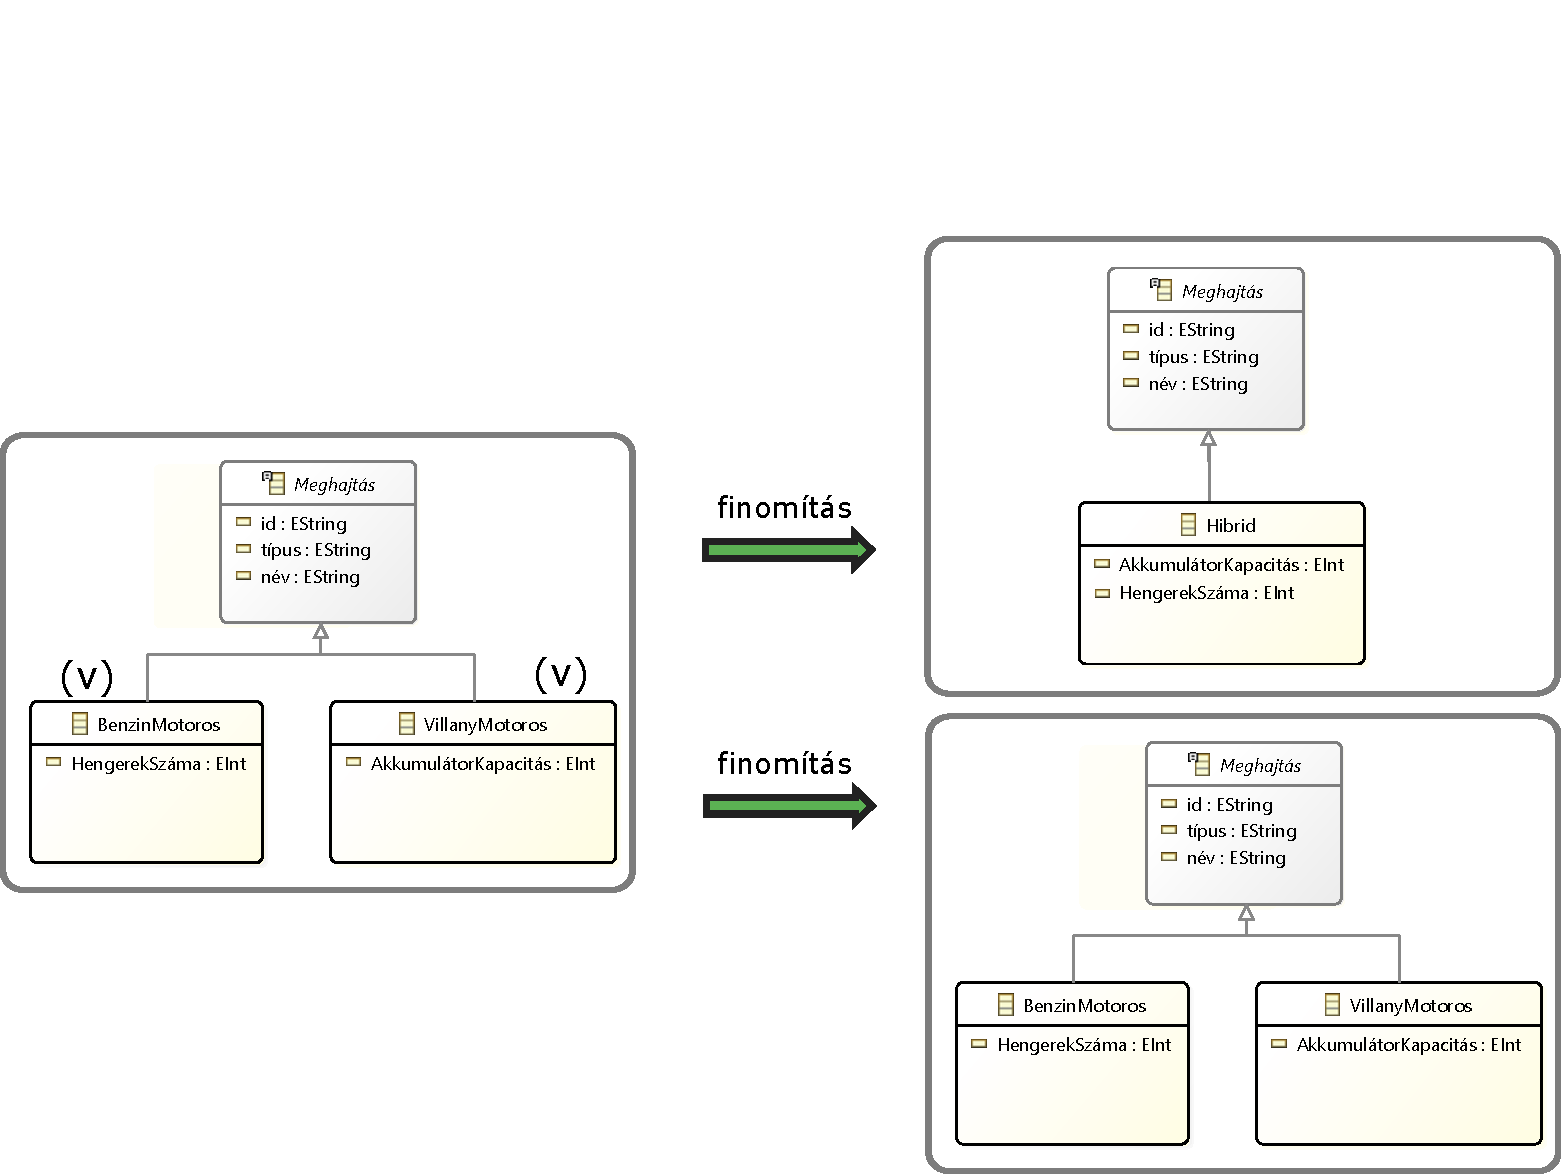
\includegraphics[width=130mm, keepaspectratio]{figures/var.pdf}
	\caption{Var részlegesség feloldása} 
	\label{var}
\end{figure}

\subsubsection{OW}
Modellezés folyamán lehet megjelölni azt, hogy a modell már végleges-e vagy sem, tehát adhatunk-e új elemeket a modellhez vagy nem. Ez a részlegesség nem a modell elemeire vonatkozik, hanem a teljes modellről árul el információt. 
